\subsection{Question 1}
    
        Consider this piece of code from a fictional C-like programming language:
        \begin{lstlisting}[language = Java , frame = trBL , firstnumber = last , escapeinside={(*@}{@*)}]                 
int x2 = 25;
while(x2>0) {
    // increment x2 by one
    x2++;
    int y = fread(file) % 10;
    if(y<=4) {
        x2 = x2 - 1;
    }
    printf("Value: %d", y);
}
        \end{lstlisting}
        
        \subsubsection{Question 1.1}
    
            \textbf{Give the symbol classes that a lexer would need to lex this code (in the course, we have seen
            some basic classes, like Identifier, or Number). Also make symbol classes for whitespaces
            (space, newline), and comments.} \\
            
            
    We will combine question 1 and 3 together, the item on the left is the symbol class, on the right we have the regular expression.
\begin{itemize}
    \item Type: \texttt{int} 
    \item Space: \texttt{$\backslash$w } 
    \item Identifier: \texttt{$[a-zA-Z][azA-Z0-9]^{*}$}
    \item Assignment op: =
    \item Number: $[0-9]^{+}$
    \item String: " .* "
    \item Special char: [$;()\{\}$]
    \item Keyword: (if$|$while)
    \item Comparison operator: [$>|\le$]
    \item Increment operator: ++
    \item Comment : // .*$\backslash$n
    \item Math operator: ($-|\%$)
    \item EOL character: ;
    \item Param separator: ,
\end{itemize}
            
        \subsubsection{Question 1.2}
            \textbf{Write the sequence of symbols ($<$Token,Attribute$>$) that a lexer would generate for this code.} \\
            
            \begin{lstlisting}[language = bash , frame = trBL , firstnumber = last , escapeinside={(*@}{@*)}]
<Type, int > 
<Identifier, x2 > 
<Assignment operator, = >  
<Number, 25 >  
<EOL character, \backslashn >  
<Keyword, while>  
<Special character, ( > 
<Identifier, x2> 
<Comparison operator, > > 
<Number, 0 >  
<Special character, ) > 
<Special character, \{ > 
<Comment, //...> 
<Identifier, x2>     
<Increment operator, ++> 
<EOL character, ;> 
<Type, int> 
<Identifier, y> 
<Assignment operator, => 
<Identifier, fread> 
<Special character, (> 
<Math operator, \%> 
<EOL character, ;> 
<Keyword, if > 
<Special character, (> 
<Identifier, y> 
<Comparison operator, \le> 
<Number, 4> 
<Special character, )> 
<Special character, \{> 
<Identifier, x2> 
<Assignment operator, => 
<Identifier, x2> 
<Math operator, -> 
<Number, 1> 
<EOL character, ;> 
<Special character, \}> 
<Identifier, printf> 
<Special character, (> 
<String, "Value: \%d"> 
<Param separator, ,> 
<Identifier, y> 
<Special character, )> 
<EOL character, ;>   
<Special character, \}> 
\end{lstlisting}
            
    \subsection{Question 2}

        \subsubsection{Question 2.1}
        \textbf{The language of a RE can be described in English words. For example, one could say that the
        RE $(0|1)^{*}1$ stands for “all binary numbers ending with a 1”. Describe the RE} 
        \begin{center}
            $(0|1)^{*}0(0|1)^{*}0(0|1)^{*}$
        \end{center}
        \textbf{in English words.} \\
        
        Any binary sequence that contains at least two zeros
        
        \subsubsection{Question 2.2}
        \textbf{Construct a RE for “all binary numbers starting with a 1 and containing exactly one pair of
        consecutive 0”.} \\
        \begin{center}
            $1 (01|1)^{*}00(1|10)^{*}$
        \end{center}

    \subsection{Question 3}
        \subsubsection{Question 3.1}
            \textbf{Draw the NFA for RE $a(bc)^{*}(d|ef)$
            Indicate which state is the initial state and which states are the final states. See the NFA in
            question 3.5 on how to indicate the initial state and final states in an NFA diagram.}

            \addimg{img/TP1/3_1.pdf}{}{NFA for $a(bc)^{*}(d|ef)$}{}
            
        \subsubsection{Question 3.2}
            \textbf{Draw the NFA for $(a|b|bc)^{*}a$ and construct the DFA. The + sign can be used to express that a pattern must appear at least one time. What would be the NFA for the RE $(a|b|bc)^{+}a$ ?}
            
            \begin{figure}%
                \centering
                \subfloat[\centering]{{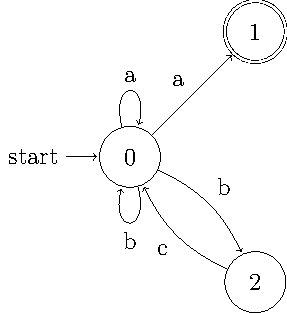
\includegraphics[width=5cm]{img/TP1/3_2a.pdf} }}%
                \qquad
                \subfloat[\centering ]{{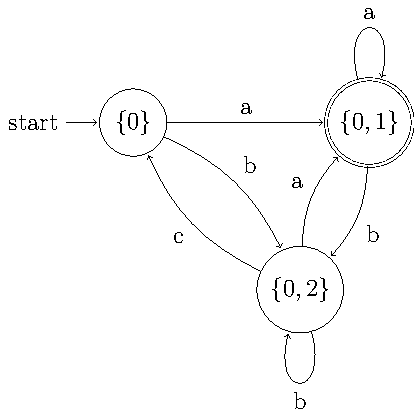
\includegraphics[width=5cm]{img/TP1/3_2b.pdf} }}%
                \caption{NFA and DFA for $(a|b|bc)^{*}a$}%
                \label{fig:example}%
            \end{figure}
           
            \addimg{img/TP1/3_2c.pdf}{}{NFA for $(a|b|bc)^{+}a$}{}

        \subsubsection{Question 3.3}
            \textbf{$\varepsilon$-transitions are very convenient if you want to combine two NFAs. Draw first the NFAs for $a^{*}$b and $c^{*}$d and then draw an NFA for ($a^{*}$b) $|$ ($c^{*}$ d) using $\varepsilon$-transitions.}

              \begin{figure}%
                \centering
                \subfloat[\centering]{{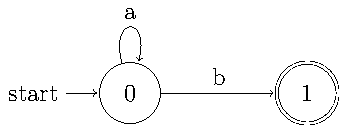
\includegraphics[width=5cm]{img/TP1/3_3a.pdf} }}%
                \qquad
                \subfloat[\centering ]{{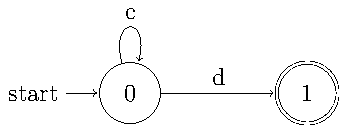
\includegraphics[width=5cm]{img/TP1/3_3b.pdf} }}%
                \caption{NFA and DFA for $(a|b|bc)^{*}a$}%
                \label{fig:example}%
            \end{figure}

           
            \addimg{img/TP1/3_3c.pdf}{}{NFA for ($a^{*}$b) $|$ ($c^{*}$ d)}{}

        \subsubsection{Question 3.4}
            \textbf{Transform the NFA for (a$^{*}$b) $|$ ($c^{*}$d) from question 3.3 into an NFA without $\varepsilon$-transitions.}

            \addimg{img/TP1/3_4.pdf}{}{NFA for (a$^{*}$b) $|$ ($c^{*}$d) without $\varepsilon$-transitions}{}

        \subsubsection{Question 3.5}
            \textbf{When dealing with NFAs with $\varepsilon$-transitions, it is useful to think about the $\varepsilon$-closure $\varepsilon$(s) of a state s, which is defined as the set of states that can be reached from that state s by doing one or several (!) $\varepsilon$-transition steps. For the below NFA over the alphabet $\Omega$ = {0,1}, give the $\varepsilon$-closures $\varepsilon$(A), $\varepsilon$(B), $\varepsilon$(C) of the states A, B, C.}

            \addimg{img/TP1/image.png}{width=0.5\textwidth}{}{}
        
            
$\varepsilon$-closures: 
\begin{center}
    \noindent $\varepsilon\{A\} = \{A, B, C\}$ \\
    $\varepsilon\{B\} = \{B, C\}$ \\
    $\varepsilon\{C\} = \{C\}$ \\
\end{center}
            \addimg{img/TP1/3_5.pdf}{}{DFA for the above graph}{}
        
        \subsubsection{Question 3.6}

            \textbf{Here is a modification of the powerset construction method seen in the course that also works with NFAs containing $\varepsilon$-transitions: \\
                • The initial state of the powerset automaton is $\varepsilon$({s0}). \\
                • The set of transitions T' of the powerset automaton is defined as:
                $\forall Q \subseteq S, c \in \Omega: (Q, c, R) \in T' for R = \varepsilon(\{t | s \in Q, (s, c, t) \in T)$
                Compare this modified method with the method that we have seen in the course. What is
                the difference?
                Transform the NFAs from question 3.3 (the combined NFA) and from question 3.5 into DFAs
                using this modified powerset construction method.}
    
            \addimg{img/TP1/3_6.pdf}{}{Combined DFA from NFAs}{}